\documentclass[
  ngerman
  ,12pt
  ,pdftex
]{article}

\usepackage{graphicx}
\usepackage{amsmath}
\usepackage{amssymb}
\usepackage{float}
\usepackage{listings}
\usepackage[ngerman]{babel}
\usepackage[utf8]{inputenc}
\usepackage[T1]{fontenc}
\usepackage{makecell}

\hyphenation{Differential-gleichung}
\hyphenation{Über-tragungs-ope-ra-tors}
\hyphenation{E/A-Dif-fe-ren-ti-al-glei-chung}

\begin{document}

\begin{titlepage}
  \begin{center}
      {\Huge \textbf{Signale und Systeme - Systemanalyse}}\\[1.5cm]
      {\Large Analyse des Systems}\\[1cm]
      {\Huge PT$_{1}$ mit negativer Verstärkung}\\[7cm]
      {\large Matrikelnummer: \textbf{8809469}}\\[0.5cm]
      {\large Matrikelnummer: \textbf{6130555}}\\[0.5cm]
      {\large Kurs: TINF21B3}\\[0.5cm]
      {\large Abgabedatum 16.12.2022}
      \vfill
  \end{center}
\end{titlepage}
\newpage
\tableofcontents
\newpage

% INPUTS

%TODO: ZEITSKALEN AUF K=100 und T=10 ändern

\section{Einleitung}    % FERTIG
% Das System, welches im Folgenden behandelt wird hat die Übertragungsfunktion
% \begin{equation*}
%   G(s)=\frac{K}{T*s+1}
% \end{equation*}\\
% und mit den Werten $K=-25$ und $T=10$ ergibt sich daraus die neue Übertragungsfunktion
% \begin{equation*}
%   G(s)=\frac{-25}{10s+1} .
% \end{equation*}\\
% Um das System analysieren zu können, haben wir das System mit den entsprechenden Werten in Simulink simuliert und die Sprungantwort betrachet.\\
% Erst danach haben wir mit Matlab gearbeitet und dort die entsprechenden Graphen plotten lassen. Mit Hilfe des Befehls \texttt{sys = tf([-25],[10 1])} haben wir unser System in Matlab erzeugt. Falls notwendig wird ein Sinus als Eingangssignal angenommen. %TODO: Stimmt das?
% % Das System ist wie folgt zu klassifizieren:
% %TODO: Klassifizierung

Das System, welches im Folgenden behandelt wird ist das $PT_1$-Glied mit negativer Verstärkung. Es wird auch Verzögerungsglied 1. Ordnung genannt. Es weist sowohl P-Verhalten als auch T-Verhalten auf. Es kann durch folgende Differentialgleichung beschrieben werden:
\begin{equation*}
  y(t)+T* \dot y(t) = K*u(t)
\end{equation*}
$K$ steht hierbei für den Proportionalitäts- bzw. Verstärkunsfaktor des Systems und $T$ ist die Zeitkonstante.\\
Bei unser System haben wir uns für die Werte $K=-25$ und $T=10$ entschieden.\\
Um das System analysieren zu können, haben wir das System mit den entsprechenden Werten in Simulink simuliert und die Sprungantwort betrachet. Erst danach haben wir mit Matlab gearbeitet und dort die entsprechenden Graphen plotten lassen.

% \section*{Vorgehen in der Systemtheorie}
% Um ein System zu beschreiben geht man im allgemeinen nach den folgenden Schritten vor:
\begin{enumerate}
    \item Detaillierungsgrad fürs Modell festlegen
    \item Physikalisches Modell erstellen
    \item Eingangs-, Ausgangs-, Zustandsgrößen festlegen (u,y,x,z)
    \item Physikalische Einheiten festlegen, ggf. Normierung in \% $\Longleftrightarrow$ Einheitenfreie Darstellung
    \item Analyse des Modells
    \begin{itemize}
        \item [a] Ruhelagen, evtl. linearisieren; Anfangswerte
        \item [b] Systemeigenschaften ermitteln
    \end{itemize}
    \item Entwurf
    \begin{itemize}
        \item [a] Ziele festlegen
        \item [b] Arbeitspunkte festlegen bzw. Trajektorien planen
        \item [c] Entwuft (Struktur, Bereich, Verfahren, Kriterium)
        \end{itemize}
\end{enumerate}

\section{Physikalische Beschreibung/Umcodierung}
Unser System weist sowohl P- als auch T-Verhalten auf und ist ein Verzögerungsglied 1. Ordnung. In der Praxis lässt sich mit diesem System beispielsweise der Kühlvorgang in einer Tiefkühltruhe beschreiben.

\vspace*{0.5cm}
\begin{center}
  \begin{tabular}{l| |l|l|l}
    & Physikalisch & Normiert   & Systemtheoretisch \\\hline\hline
    & & & \\
    Eingang   & (Kühl-)Energie  & $Wh$ & $u$ \\
    Ausgang   & Temperatur      & °C                & $y$ \\
    Zustand   & Temperatur      & °C                & $x_{1}$ \\
    Parameter & \makecell[l]{Niedrigste Temperatur des\\ Kühlgerätes,\\Leistung des Kühlgerätes}                & °C, $\frac{BTU}{h}$    & $K$, $T_{1}$ \\
  \end{tabular}
\end{center}
\vspace*{0.5cm}
\noindent{}Die Wahl der Zeitkonstante $h$ ist naheliegend, da Kühlgeräte die Temperatur normalerweise nur langfristig (im Stundenbereich) ändern können.\\
Die Normierung und Festlegung der Einheiten ist wichtig, damit die Plots mit den richtigen Zeitskalen beschriftet werden können.

%Eine Normierung des Eingangs auf den Bereich 0 bis 100% ist häufig sinnvoll, da dann die statische Verstärkung angibt, auf welchem Endwert ich bei 100% (also max. Eingang) lande (bei P-Gliedern).

%ACHSEN DER PLOTS RICHTIG BESCHRIFTEN, damit die Einheiten richtig abgelesen werden können!!!! Beschriften: [t]=s oder t in s oder t/s oder "Zeit in Sekunden"

%Matlab Befehle: labelx/yaxis: entweder t/s oder t in s/sec./Sekunden oder Zeit in Sekunden

  %CHRIS:
  % \begin{tabular}{l|l|l|l}
        %     \centering
        %         0 & physikalische Darstellung & normierte Darstellung & systemtheoretische Darstellung  \\ \hline
        %         Eingang & Durchfluss Wasserhahn & 0-100\% & u \hline
        %         Ausgang & Höhe des Wassers & V/V_ges & y \hline
        %         Zustand & Höhe des Wassers & cfaef & x_1, x_2 ... je nach Ordnung \hline
        %         Parameter & Masse, Länge,Trägheitsmoment, Kapazität, Induktivität & T, $T_D$, D
        % \end{tabular}

\section{Übertragungsfunktion}    % FERTIG
\input{inputs/2.1_Übertragungsfunktion.tex}

\section{Zustandsraumbeschreibung (implizite Systembeschreibung)}
\subsection{Allgemein}
Um die Zustandstaumdarstellung zu bestimmen, werden die Matrizen $A$, $B$, $C$ und $D$ benötigt. Diese stehen wie folgt mit dem System im Zusammenhang:
\begin{equation*}
  \dot\vec{x} = A\vec{x} + B\vec{u}
\end{equation*}
\begin{equation*}
  y = C\vec{x} + D\vec{u}
\end{equation*}
Die Zustandsübergangsfunktion beinhaltet die Systemmatrix $A$ und die Eingangsmatrix $B$ und gliedert sich in den Eigenvorgang sowie den erzwungenen Vorgang. Im Folgenden ist diese Übergangsfunktion dargestellt:
\begin{equation*}
  \varphi (t,t_0,x_0,u) = e^{A(t-t_0)}x(t_0)+\int_{t_0}^{t}e^{A\tau }Bu(t-\tau )d\tau
\end{equation*}
Der Übertragungsoperator bezieht zusätzlich die Ausgangsmatrix $C$ und die Durchgriffsmatrix $D$ mit ein.
\begin{equation*}
  \psi (t,t_0,x_0,u_{[t_0,t)}) = Ce^{A(t-t_0)}x(t_0)+\int_{t_0}^{t}Ce^{A\tau }Bu(t-\tau )d\tau + Du(t)
\end{equation*}
\vspace*{0.5cm}
Die Matrizen $A$, $B$, $C$, $D$ lassen sich in Matlab wie folgt generieren:\\
\hspace*{0.5cm}\texttt{sys = tf([-25],[10 1])}\\
\hspace*{0.5cm}\texttt{ss(sys)}



\subsection{Unser System}
Da Matlab mit den obigen Befehlen ungünstige Werte für $B$ und $C$ liefert, leiten wir die Werte aus der nach $\dot y$ umgestellten Differentialgleichung (Herleitung im Kapitel E-/A-Differentialgleichung) unseres Systems her: 
\begin{equation*}
  \dot y(t)= \frac{1}{10}(-y(t)-25u(t))
\end{equation*}
Wird umgeformt zu:
\begin{equation*}
  \dot y(t)= -\frac{1}{10}y(t)-2,5u(t)
\end{equation*}
Da unser System ein System 1. Ordnung ist, lassen sich aus dieser Form direkt die Werte für $A$, $B$, $C$ und $D$ ablesen. Somit ergeben sich folgende Werte:
\begin{equation*}
  A = [-0,1]; B = [-2,5]; C = [1]; D = 0
\end{equation*}
Für unser System wählen wir den Anfangswert x(0) = 0.
Somit lässt sich die folgende Zustandsraumdarstellung herleiten:
\begin{equation*}
  \dot \vec{x} = [-0.1][x_1] + [-2.5]u
\end{equation*}
\begin{equation*}
  y = [1][x_1] + [0]u
\end{equation*}

\section{Ein-/Ausgangsdifferentialgleichung}
\subsection{Allgemein}
% Durch Überkreuzmultiplikation kann man von der Übertragungsfunktion auf die Eingangs- / Ausgangsdifferentialgleichung schließen. Von der Form:\\
Die Eingangs-/Ausgangsdifferentialgleichung kann aus der Übertragungsfunktion durch Rücktransformation aus dem Laplace-Bereich bestimmt werden:
\begin{equation*}
  G(s) = \frac{Y(s)}{U(s)} = \frac{K}{T_1*s+1}
\end{equation*}
Durch Überkreuzmultiplikation gelangt man zu:
\begin{equation*}
  Y(s)*(T*s+1) = U(s)*K
\end{equation*}
Durch Ausklammern erhält man:
\begin{equation*}
  T*Y(s)*s + Y(s) = U(s)*K
\end{equation*}
Die lineare Differentialgleichung wird durch Umwandlung mit Hilfe der inversen Laplace-Transformation ermittelt:
\begin{equation*}
  T* \dot y(t) + y(t) = K * u(t)
\end{equation*}
Zur Vereinheitlichung der Ableitungen $y(t)$ werden die Koeffizienten mit dem Buchstaben a dargestellt.
Auf der rechten Seite werden die Koeffizienten der Ableitungen von $u(t)$ mit $b_0$ und fortlaufend nummeriert:
\begin{equation*}
  a_1\dot y(t)+a_0y(t) = b_0u(t)
\end{equation*}
Die höchste Ableitung von $y$ wird vom Koeffizienten freigestellt, in dem alle Terme der Gleichung auch durch $a_1$ dividiert werden und nach der höchsten Ableitung aufgelöst wird:
\begin{equation*}
  \dot y(t)= \frac{1}{a_1}(-a_0y(t) +b_0u(t))
\end{equation*}

\subsection{Unser System}
Werden die obigen Schritte auf die Übertragungsfunktion unseres Systems angewendet, erhält man:
\begin{equation*}
  G(s)=\frac{Y(s)}{U(s)}=\frac{-25}{10s+1}
\end{equation*}
\begin{equation*}
  Y(s)*(10s+1) = -25*U(s)
\end{equation*}
\begin{equation*}
  10*Y(s)*s + Y(s) = -25*U(s)
\end{equation*}
\begin{equation*}
  10 \dot y(t) + y(t) = -25u(t)
\end{equation*}
Nach $\dot y(t)$ umformen:
\begin{equation*}
  \dot y(t)= \frac{1}{10}(-y(t)-25u(t))
\end{equation*}

\section{Explizite Darstellung des Übertragungsoperators}
\input{inputs/5_Explizite Darstellung des Übertragungsoperators.tex}

\subsection*{Zustandsraumbeschreibung in Übertragungsfunktion}
\input{inputs/E2_ZustandsraumbeschreibunginÜbertragungsfunktion.tex}

\section{Zusammenhänge der Funktionen $G(s)$, $g(t)$, $h(t)$ und $\frac{G(s)}{s}$}
Die Übergangsfunktion stellt die Veränderung des Signals innerhalb des Systems als Funktion dar. Diese
kann durch Integrieren aus der Gewichtsfunktion (später dargestellt) gebildet werden. Dafür nutzt man wie
in den folgenden Abbildungen dargestellt den Laplace-Bereich, da nicht alle Funktionen einfach integriert
werden können.
\vspace*{0.5cm}
\begin{figure}[H]
    \begin{center}
        \fbox{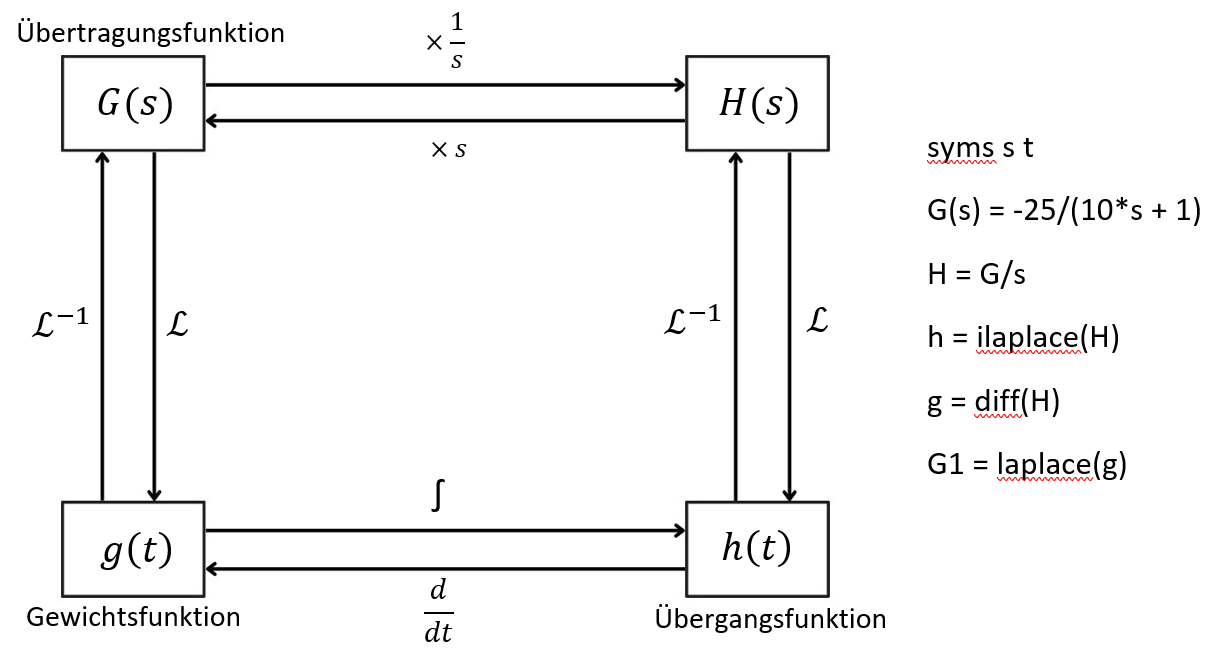
\includegraphics[width=13cm]{image/funktionen-fertig.png}}
    \end{center}
\end{figure}
\vspace*{0.5cm}
Der Vorteil der Laplace-Transformation ist, dass sich komplizierte Operationen der Analysis, wie bspw. Faltung, durch einfache Multiplikation im Laplace-Bereich äußern. Sofern man in der Klasse der linearen Zeitinvarianten Systeme (LTI) ist, sind die Laplace-Transformierten rationale Funktionen (Polynom/Polynom). Somit können Polynomdivision, Patialbruchzerlegung usw. angewendet werden.

\section{Übergangsfunktion/Sprungantwort}
\input{inputs/7_Übertragungsfunktion-Sprungantwort.tex}

\section{Gewichtsfunktion/Impulsantwort}
%CHRIS: Antwort auf einen Delta-Impuls.
Die Gewichtsfunktion kann aus der Übertragungsfunktion durch Ableiten erhalten werden.
Alternativ kann die Gewichtsfunktion aus der Übertragungsfunktion durch Differention gewonnen werden.
%Die Lösung von Matlab ist zwar die gleiche, aber in einer anderen Darstellung. Sollte Matlab einen zu langen Ausdruck ausgeben, kann der Befehl simplify(ans) verwendet werden, um den Ausdruck zu vereinfachen.
...
\subsection{Parametrische Darstellung} %NICHT SICHER
Die Parametrische Darstellung der Gewichtsfunktion $g(t)$ erhält man, indem man die Laplace-Rücktransformierte der Übertragungsfunktion bildet. Das macht man wie folgt: 
%syms s -> G(s)=bspw. 3*s/(1+9*s + 20*s^2) -> ilaplace(G(s)) -> t=[0;0.1;10] -> plot(t, Antwort der parametrischen Darstellung) (Da t ein Vektor ist, muss man beim Multiplizieren das Punktprodukt (Hadamad-Produkt) .* verwenden) (Alternativ kann man das mit dem fplot befehl machen, da spart man sich das Hadamad-Produkt) -> xlabel (Mit den Befehlen xlabel und ylabel kann man die Achsen beschriften) -> ylabel Gewichtsfunktion
%texttt{sys=tf([..][..])}
%texttt{syms s \\ ...}
Das macht man wie folgt:
\texttt{syms s}\\
\texttt{syms t}\\
\texttt{G(s)=-25/(10*s+1)}\\
\texttt{g(t)=ilaplace(G(s))}\\
Matlab liefert hier $g(t)=-\frac{5*e^{\frac{-t}{10}}}{2}$
\subsection{Nichtparametrische Darstellung}
\subsubsection{Plot mit Matlab}
Mit der parametrischen Darstellung kann die Gewichtsfunktion in Matlab geplottet werden.
Hier graphisch dargestellt:\\
\texttt{t=[0:0.1:50]}\\
\texttt{t,-(5*exp(-t/10))/2}

\begin{figure}[H]
    \centering
    \includegraphics[width=5cm]{image/ImpulsantwortPlotinMatlab.eps}
    \caption{Impulsantwort: Plot in Matlab}
\end{figure}


\subsubsection{Plot mit Step-Funktion}
Den selben Plot bekommt man auch über die Matlab \texttt{impulse} Funktion\\
\texttt{sys=tf([-25], [10 1])}
\texttt{impulse(sys)}
\begin{figure}[H]
    \centering
    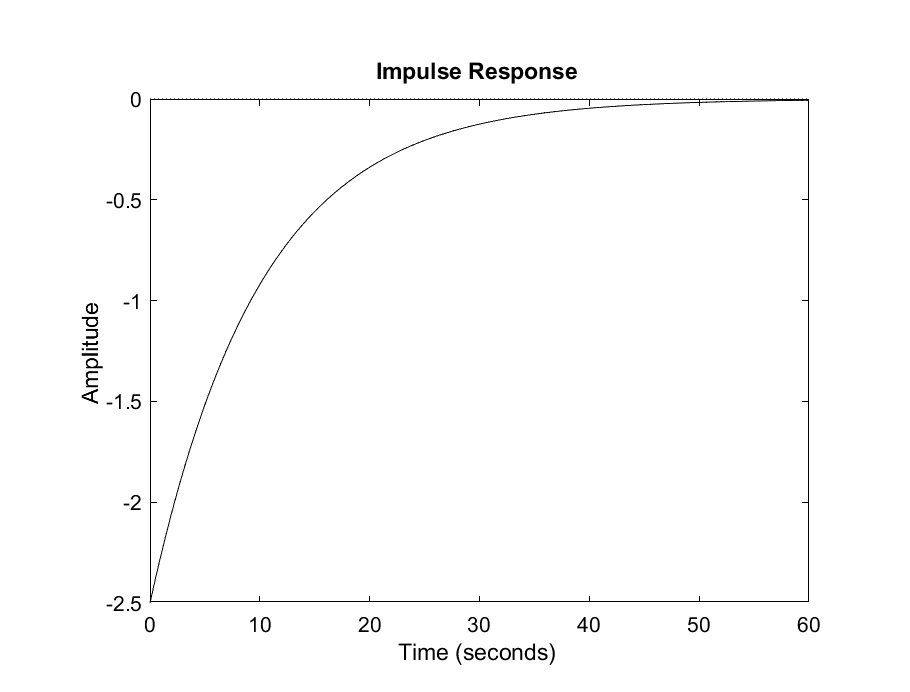
\includegraphics[width=5cm]{image/ImpulsantwortPlotmitImpulsFunktion.eps}
    \caption{Impulsantwort: Plot mit Impuls Funktion}
\end{figure}

\subsubsection{Plot mit Simulink}
...

\section{Frequenzgang}
\subsection{Parametrische Darstellung}
Den Frequenzgang erhält man indem man die komplexe Variable $s$ durch iOmega ($i\omega$) ersetzt. \\
Das ist gleichbedeutend mit einem Schnitt der komplexen Funktion $G(s)$ entlang der imaginären Achse.
Damit wird jeder Kreisfrequenz $\omega$ eine komplexe Zahl $G(i\omega)$ zugeordnet. 
\\
\\
Bedingt durch den Schnitt hat der Frequenzgang eine geringere Aussagekraft als die Übertragungsfunktion. 
Die Bedeutung des Frequenzgangs ergibt sich aus der Tatsache, dass das stationäre Verhalten des Systems auf eine sinuidale Anregung beschrieben wird.\\
\\

Sei $u(t) = sin(\omega t)$, so ist $y_{stat}(\dot{t})$ %TODO: KONTROLLE
, dh. das Ausgangssignal nach Abklingen der Anfangswerte durch:
\begin{equation*}
    y_{stat}(t)=A*|G(i\omega )|sin(\omega t + \phi (G(i\omega )))
\end{equation*}

gegeben. %TODO: KONTROLLE und Block
%Der Frequenzgang liefert formal weniger Aussagen als die Übertragungsfunktion, da er nicht alle $s$ betrachtet, sondern nur die $s$, die auf der imaginären Achse liegen.\\
%Experimentell könnte der Frequenzgang durch die folgende Simulink-Schaltung aufgenommen werden. 
%TODO: Schaltung einfügen
%Man stellt eine Frequenz ein und schaut am Ausgang die Amplitudenverstärkung und die Phasenverschiebung an. Hat der Eingangssinus die Amplitude 1, kann ich die Verstärkung am Ausgang direkt ablesen. Den erhaltenen Punkt trägt man in das Bode-Diagramm ein. Danach wiederholt man das Experiment mit einer anderen Frequenz. Hat man genügend Punkte, so verbindet man diese und erhält das Bode-Diagramm. Ebenso wie wir an den Verläufen der Sprungantwort auf die Differentialgleichung schließen konnten, können Experten aus den Verläufen des Bode-Diagramms auf den Frequenzgang (und damit auf die Übertragungsfunktion und damit auf die Differentialgleichung) schließen.\\
%Die Phasenverschiebung kann selbstverständlich auch mit Computeralgebra ausgerechnet werden.
\subsection{Nichtparametrische Darstellung}
Experimentell kann der Frequenzgang durch folgende Simulink Schaltung aufgenommen werden:
\begin{figure}[H]
    \centering
    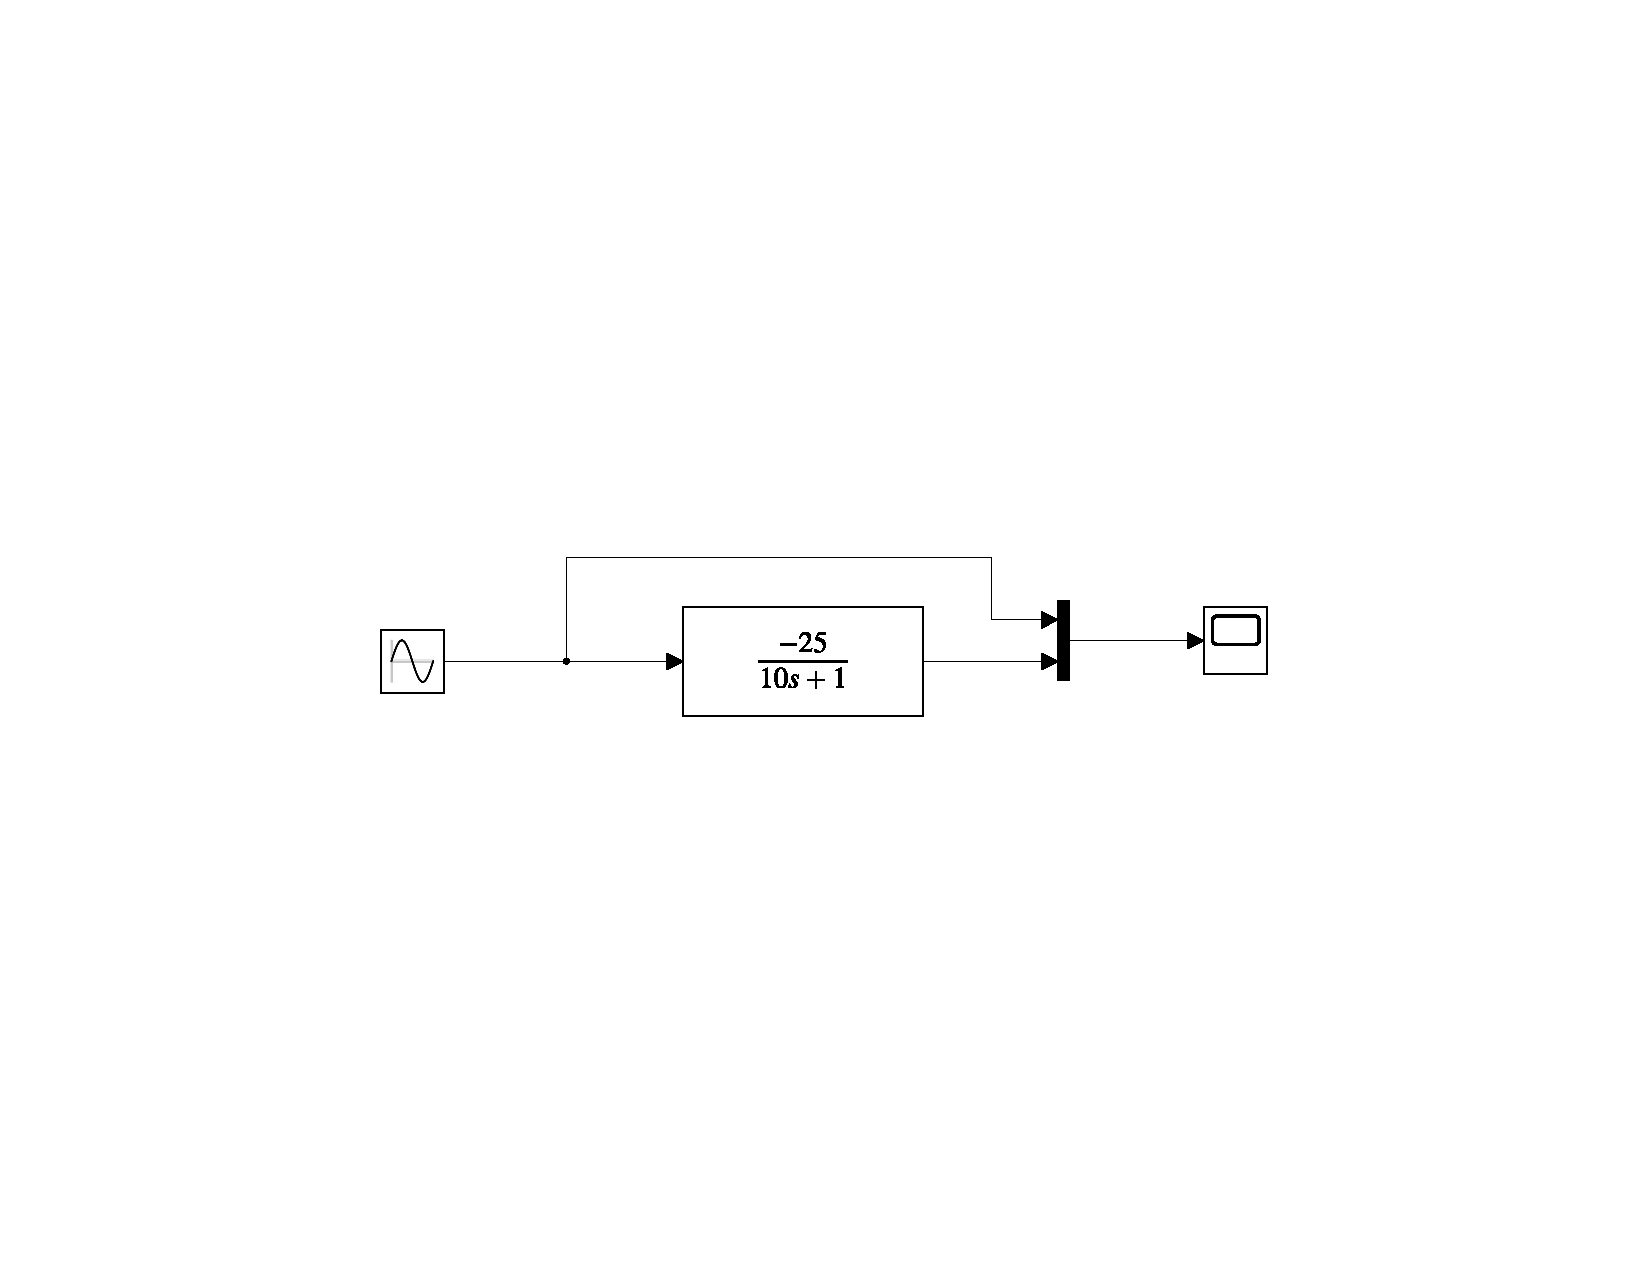
\includegraphics[width=8cm]{image/FrequenzgangSchaltung.pdf}
    \caption{Frequenzgang: Simulink Schaltung}
\end{figure}
\begin{figure}[H]
    \centering
    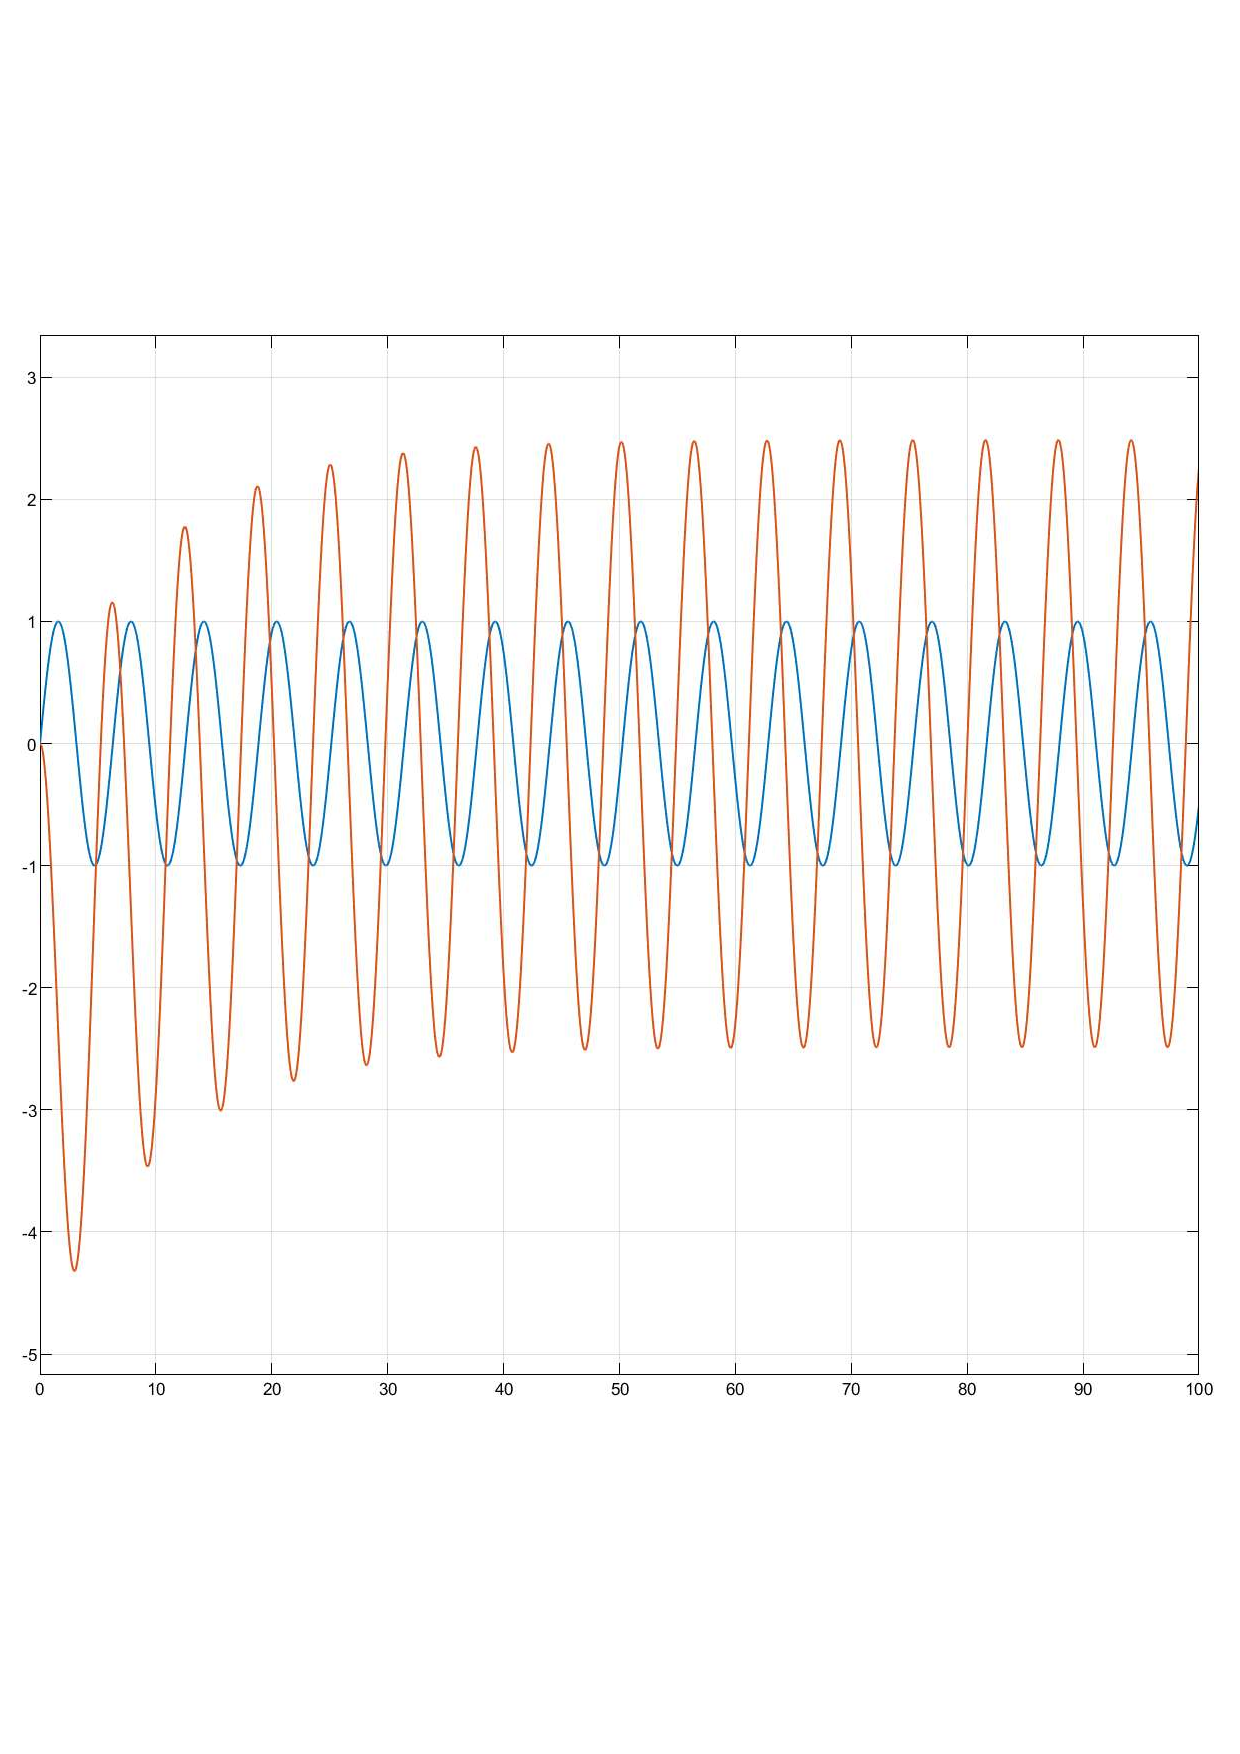
\includegraphics[width=8cm]{image/FrequenzgangAusgang.pdf}
    \caption{Frequenzgang: Plot mit Simulink}
\end{figure}

Am Eingangssinus wird eine Frequenz eingestellt und am Ausgang die Amplituden-
Verstärkung und die Phasenverschiebung betrachtet.
Hat der Eingang die Amplitude 1, kann man die AusgangsverstÄrkung direkt
ablesen.
Das Experiment wird mit verschiedenen Frequenz wiederholt und die jeweiligen
Ergebnisse werden dabei als Punkte in die folgenden Diagramme eingetragen.
\subsubsection{Nyquist-Plot (Ortskurve)}
Beim Nyquist-Plot ist auf der X-Achse der Realteil der gemessenen Punkte
und auf der Y-Achse der Imaginärteil, bei steigender Frequenz $\omega$ zu sehen.
Dieser lässt sich in Matlab mit folgendem Befehl generieren:\\
\texttt{nyquist(sys)}
\begin{figure}[H]
    \centering
    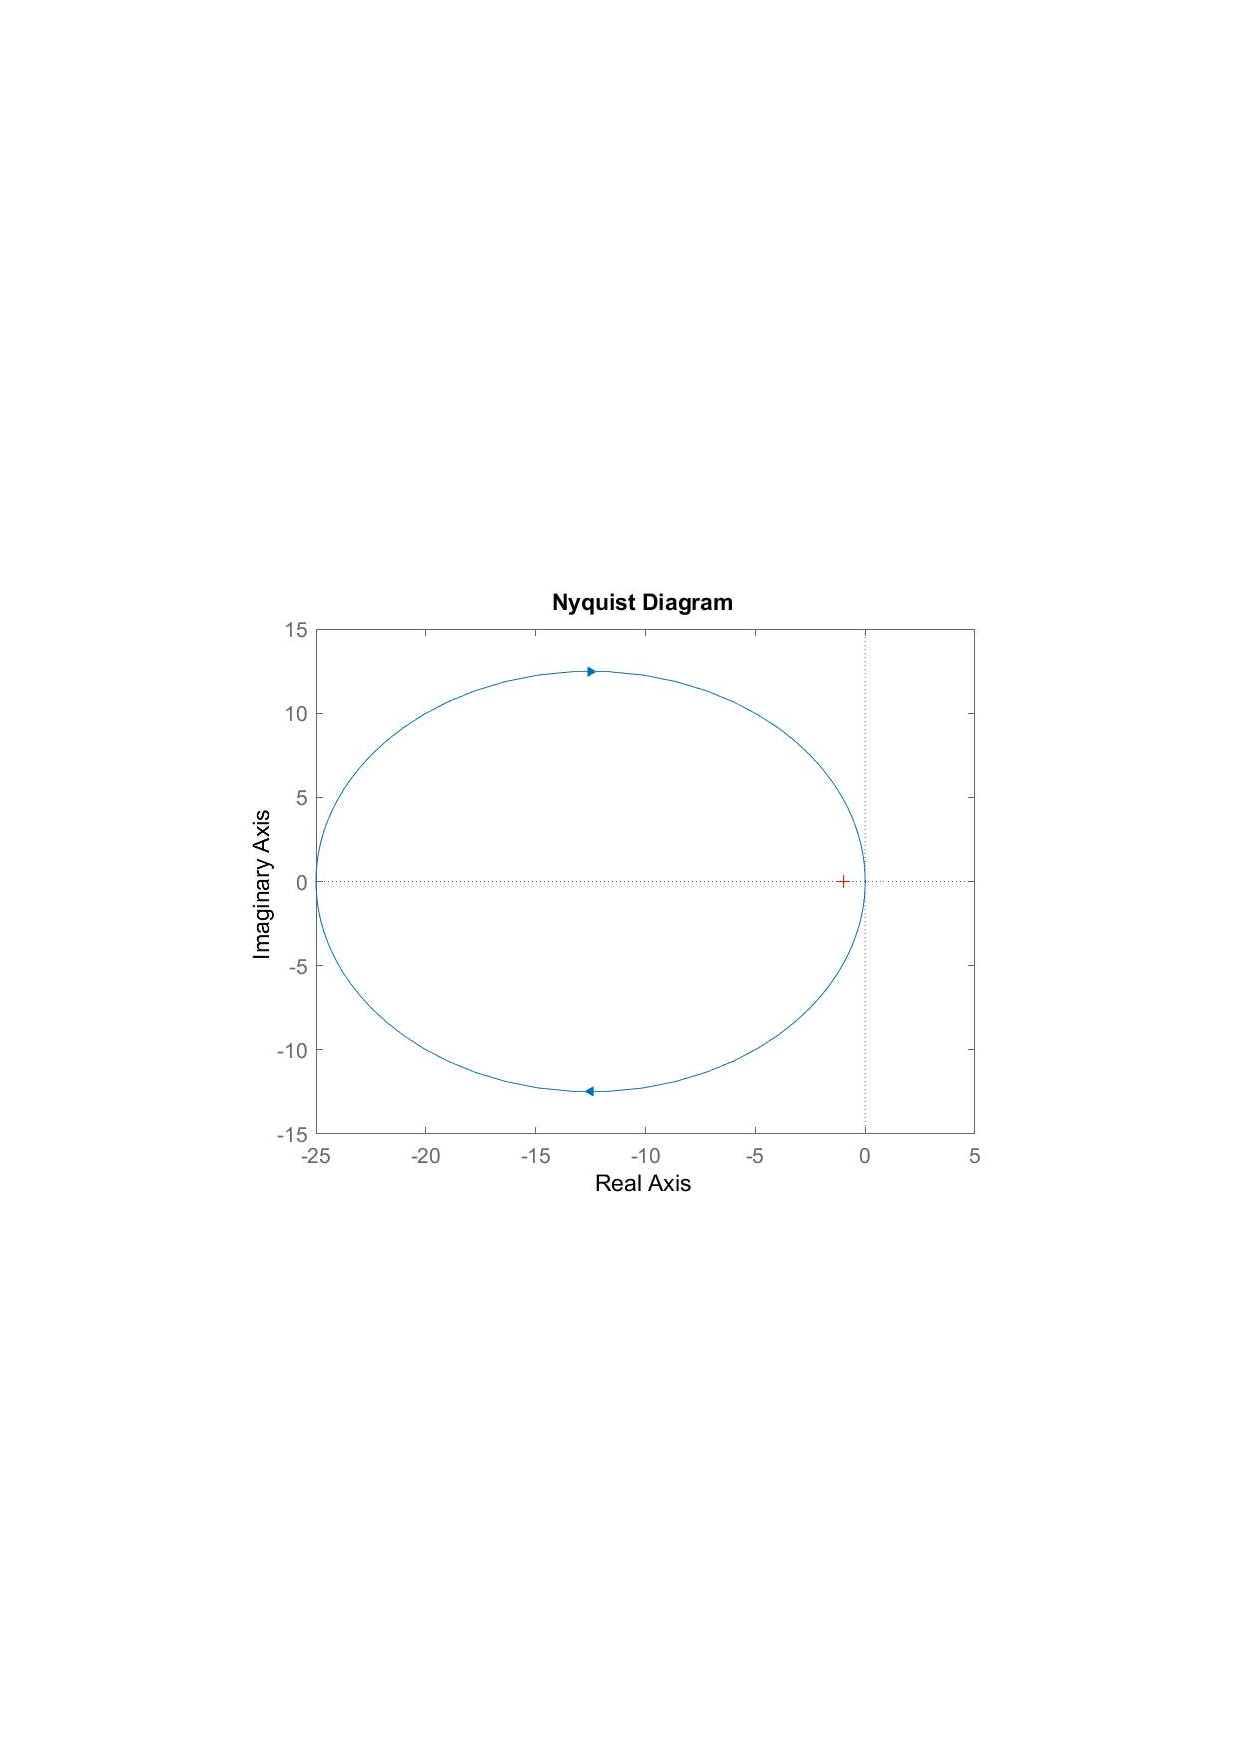
\includegraphics[width=8cm]{image/NyquistPlot.pdf}
    \caption{Frequenzgang: Nyquist Plot}
\end{figure}
\subsubsection{Bode-Plot}
In Matlab lässt sich der Bode Plot mit dem Befehl\\
\texttt{bode(sys)}\\
erzeugen.
\begin{figure}[H]
    \centering
    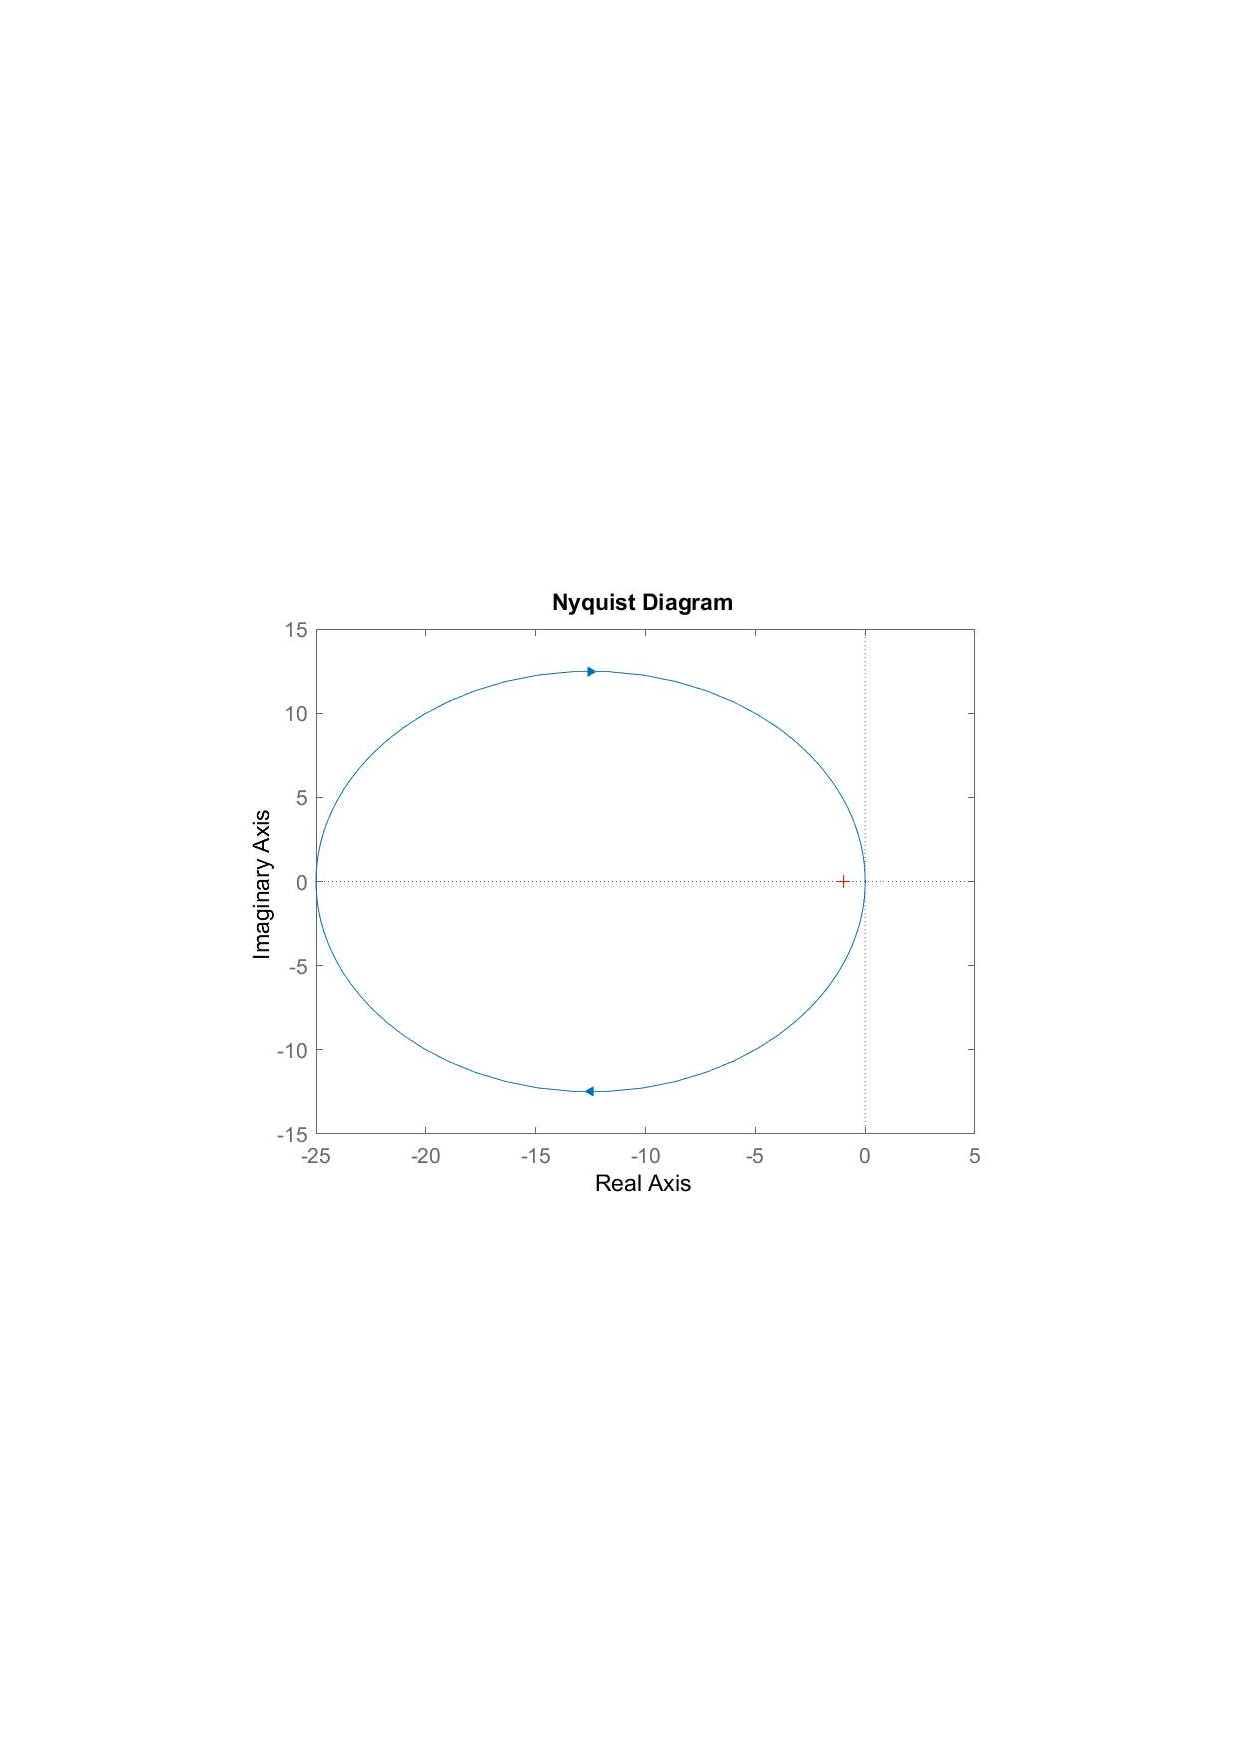
\includegraphics[width=8cm]{image/NyquistPlot.pdf}
    \caption{Frequenzgang: Bode-Plot}
\end{figure}

\section{Pol-Nullstellen-Plot}
Der Pole-Zero-Plot stellt die Pole und Nullstellen der Übertragungsfunktion in der komplexen Ebene dar. Pole werden durch ein Kreuz dargestellt, Nullstellen durch einen Kreis. Ein Doppelpol wird durch ein Doppelkreuz und eine Nullstelle durch einen Doppelkreis dargestellt. Der PZP enthält keine Informationen mehr über die statische Verstärkung. Aus dem PZP lassen sich Eigenschaften wie Stabilität und Minimalphasigkeit ablesen. So ist ein System stabil, wenn alle Pole in der linken offenen Halbebene liegen. Es ist instabil, sobald ein Pol auf der rechten Halbebene liegt. Es ist grenzstabil, wenn keine Pole in der rechten Halbebene liegen aber einige auf der imaginären Achse liegen. Ein System ist minimalphasig, wenn alle Nullstellen in der offenen linken Halbebene liegen. Es ist nicht minimalphasig, sobald eine Nullstelle auf der rechten Halbebene liegt. Und letztlich ist es schwachminimalphasig, wenn keine Nullstelle auf der rechten Halbebene liegt, aber Nullstellen auf der imaginären Achse auftauchen.\\
In Matlab lässt sich der Pol-Nullstellen-Plot mit folgendem Befehl erzeugen:\\
\hspace*{0.5cm}\texttt{pzplot(sys)}\\
Das Ergebnis dieses Befehls ist in der nachfolgenden Abbildung dargestellt:
\begin{figure}[H]
    \centering
    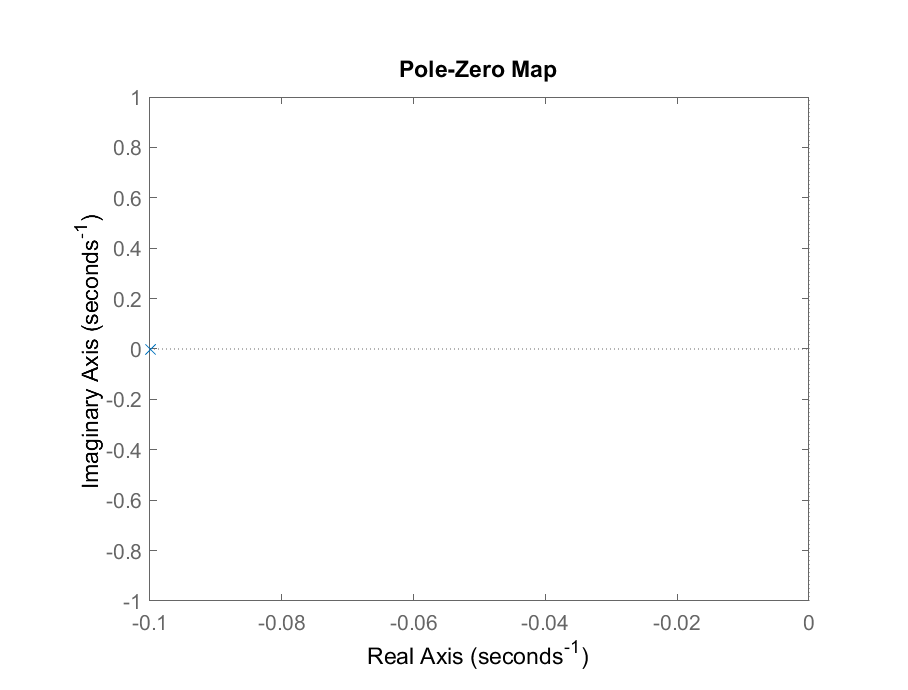
\includegraphics[width=10cm]{images_2/Rest/pzp.eps}
    \caption{Pol-Nullstellen-Plot}
\end{figure}

\section{Statische Kennlinie}
In der statischen Kennlinie wird der Ausgang über dem Eingang dargestellt. Bei einem linearen System (unten $u$ oben $y$) ist die statische Kennlinie eine Ursprungsgerade, deren Anstieg der statischen Verstärkung entspricht. Die statische Verstärkung $K$ kann aus $G(0)=K$ berechnet werden. Sie ist bei Systemen mit D-Verhalten 0 und bei Systemen mit I-Verhalten unendlich. Mit anderen Worten, Systeme mit I-Verhalten haben keine Kennlinie. In der statischen Kennlinie ist keinerlei Dynamik zu erkennen. Die Information über Pole, Nullstellen, etc. fehlt. Sie ist somit die schwächste der Modellbeschreibungen. Gleichwohl ist sie einfach zu bestimmen. Man stellt einen konstanten Wert $u$ ein, wartet bis die Eigenvorgänge abgeklungen 
%(bis es eingeschwungen ist) 
sind und liest den $y$-Wert ab. Diesen Punkt trägt man in das Diagramm ein und wiederholt das ganze für mehrere Punkte. In der Praxis werden sich häufig nicht ideale Geraden ergeben. Bei Öfen verringert sich der Anstieg beispielsweise bei hohem $u$. Der Praktiker ließt aus der statischen Kennlinie ab, wie gut seine Annahme eines linearen Modells ist. Sie ist gut in einem Bereich, in dem eine Geradenapproximation akzektabel ist (wenn sie einer Gerade ähnelt). Bei einem Mehrgrößensystem mit zwei Eingängen und zwei Ausgängen wählt man häufig die folgende Darstellung: Entweder zwei Einzeldiagramme, oder ein Verbunddiagramm (zwei Eingänge ein Ausgang: Üblicherweise keine 3D-Darstellung, sondern Transistorkennlinien). Bei Systemen mit zwei Eingängen 
%wird häufig eine Eingangsvariable durch Kennlinienscharen diskretisiert/
wählt man häufig die Darstellung mit Kennlinienscharen, wobei beispielsweise $u_{1}$ die reellen Zahlen darstellt und $u_{2}$ den Scharparameter darstellt.
%Indem man alle Ableitungen gleich Null setzt und eine Beziehung zwischen den y und u herstellt. Gegebenenfalls muss x eliminiert werden (lineares Gleichungssystem).


\end{document}



%Vorteil Übertragungsfkt/Laplace-Transformation: Komplizierte Operationen in der Analysis wie Faltung äußern sich im Laplace-Bereich durch einfache Multiplikation. Sofern man in der Klasse der linearen Zeitinvarianten Systeme (LTI) ist, sind die Laplace-Transformierten rationale Funktionen (Polynom/Polynom) -> Damit gehen Polynomdivision, Patialbruchzerlegung usw.

%TODO: Linearisierung:
%Nachdem man die Ruhelagen berechnet hat kann man um jede einzelne Ruhelage das System linearisieren. In der Folge entsteht ein lineares System, welches für kleine Abweichungen um die Ruhelage Gültigkeit hat. Man nennt dieses auch die Variationsgleichung oder einfach auch linearisiertes System. Das linearisierte System ist deutlich einfacher zu behandeln, da sich z.B. über Eigenwerte Aussagen zur Stabilität der Ruhelage treffen lassen. Vorgehen:
%Im Falle eines SiSo-Systems ist f(x) die Jacobi-Matrix an der Ruhelage und f_u der Eingangsvektor.